% Chapter 2

\chapter{Background and Related Work} % Main chapter title

\label{Chapter2} % For referencing the chapter elsewhere, use \ref{Chapter2}

This chapter serves to introduce key and essential concepts of robotics system benchmarking and SLAM systems. 
Prior knowledge of SLAM and relevant technical understanding is not presupposed for reading this chapter, so the internal workings of specific SLAM systems, including the applied mathematics and codes, will not be elaborated. 
Rather, we introduce modular conceptualization of robotics system benchmarking and SLAM to assist the reader in understanding the structure of our filtering system. 
In-depth knowledge of SLAM systems is not strictly required, but we reference some of them in evaluating the results of our testing and experiments.

%----------------------------------------------------------------------------------------
%	SECTION 1
%----------------------------------------------------------------------------------------

\section{Robotics System Benchmarking}

\subsection{Background}
Collaborative operations between man and machine has not only improve productivity, but also in some cases provide solutions not yet available to humans alone (disaster search and rescue robots) \cite{madhavan2009benchmarking}. 
Co-development between engineering and computer sciences have started to lay the foundations for mechanical hardware and software systems of generic and domain-specific robots. 
Yet without standardization, developing robotic technologies becomes not only ineffective, but also unprofessional and dangerous. 
For example, with proper standardization of video medium, there was a wide confusion and frustration of choosing HD DVD or Blue Ray for home-video appliance among consumers. 
On the other hand, successful standardization would bring synergies among different fields and cohesion between various research projects. 
For instance, the immense progress in the wireless communication technology has largely attribute to the establishment of widely accepted industrial standards such as IEEE 802.11. \cite{madhavan2009benchmarking}.

\subsection{Methodology}
Objective performance evaluation is required for each field of robotic systems to continue the progress of research and to facilitate the acceptance of robotic technologies. 
Yet it is not a trivial task to ensure that the evaluation is repeatable, unambiguous and holistic. Specifically, in the field of robot navigation and mapping, distinct research projects may take different approaches to measure the accuracy of mapping \cite{sturm2012benchmark} \cite{handa2014benchmark}. 
However, even if a standard for accuracy comparison do exists, this benchmark is not enough to characterise the mapping system as a whole: there are still considerations such as energy consumption and performance. 
Recently, there has been initiative, such as RoboBench, that intends to construct a framework that allows researchers to holistically benchmark all aspects of robotic systems and form a set of comparable, reproducible measure. 
Hence, when building a benchmarking framework for robots, systematic approach needs to be taken to account the cost of computing over the task, the performance of robotics algorithms, as well as the costs incurred in infrastructure such as energy and networks \cite{weisz2016robobench}.

To ensure the completeness of Robotic system benchmarking, two aspects of benchmark categories need to be considered: the method that determines how we benchmark, and the focus that determines what we benchmark \cite{del2006benchmarks}. 
In general, there are two methods of benchmarking: analytical approach that concerns with evaluation of a robotics system on its own, and functional approach that test how a system solves a specific problem. 
Similarly, in terms of the focus, there are also two targets of benchmarking: component – evaluation on one specific part of the system, and system – evaluation on the overall system. 
By combining these criteria, we are able to form a matrix of our robotics benchmark system:


	\begin{table}[h]
		\centering
		\caption{\label{tab:robobench}Robotics benchmark matrix.}
		\begin{tabular}{|c|c|c|}
	 	\hline
		\rotatebox{90}{Analytical \textcolor{white}{hold}} & \makecell{ 1 \\ \\ \\ \\ } & \makecell{ 3 \\ \\ \\ \\ } \\ 
		\hline
		\rotatebox{90}{Functional \textcolor{white}{hold}} & \makecell{ 2 \\ \\ \\ \\ } & \makecell{ 4 \\ \\ \\ \\ } \\ 
		\hline
		\cellcolor[HTML]{000000} & Component (filter) & System (SLAM system) \\ 
		\hline
		\end{tabular}
	\end{table}


\subsection{Application}
In the case of our filtering system in the SLAMBench, to apply the framework of holistic evaluation, we identify four potential areas of benchmark that we intend to explore based on Table \ref{tab:robobench}.
\begin{enumerate}
	\item \textbf{Use the same dataset and apply different filters.} \\
	Since we already understand the task of each filter, this process merely allows us to observe whether data set has been correctly filtered.
	\item \textbf{Use different datasets and apply the same filter.} \\
	\textit{Targeting problem:} Supposed task of a filter
\\
	\textit{Benchmark purpose:} what is the performance of a filter at carrying out its filtering tasks.
	\item \textbf{Use the same filter and apply to different SLAM systems.}
\\
	\textit{Benchmark purpose:} observe how the same filtering technique would impact different SLAM systems. 
	\item \textbf{Use different filters and apply to the same SLAM systems.} \\
	\textit{Targeting problem:} SLAM benchmarking outcome (accuracy, computational speed, energy consumption)
\\
	\textit{Benchmark purpose:} how does different filters affect a specific SLAM system? What is the optimal filtering technique for a SLAM system?
\end{enumerate}

These benchmarking methods are designed to be holistic to test the filtering system and its correlation with the SLAM systems. 
In addition, to ensure that the benchmarking results are repeatable, only minimal configuration should be required throughout the system. 
Therefore, modularization of each part of the system, where every module functions independently from each other, is the key to protect the integrity of the whole benchmarking system. 
Further details with regards to benchmarking and system design are included in the following chapters.

\subsection{Extension: Reinforcement Learning}

Beyond the purpose for standardizing industrial performance for robotic tasks, what makes benchmarking ever more essential and exciting is the emergence of reinforcement learning. 
Similar to the SLAM problem and numerous other continuous control robotic tasks, in the paradigm of reinforcement learning, a robot is not told which action to take, but instead “must discover which actions yield the most reward by trying them out” \cite{sutton2018reinforcement}. 
By doing so, the robot will need to maximize a numerical reward signal. 
In the case the SLAM problem, such reward signal could be accuracy of trajectory, power consumption, speed or combined metrics. 
However, reinforcement learning does not stop at the end of benchmarking. 
The result of the benchmark will then be fed back to the computational loop to further optimize the efficiency of robotic actions. 

This evolutionary learning method seems promising as it may finally address some of the robotic problems that have been solved theoretically, but still lack real-world applicability. 
However, researchers quickly realize the problem of applying reinforcement learning to robotic tasks: \textbf{lack of benchmark tasks and supporting tools} \cite{mahmood2018benchmarking}. 
For more advanced tasks beyond SLAM such as path planning, robots not only needs to map and localize itself, but also need to reach a certain goal through optimum path \cite{klancar2017path}. 
Robots need to actively make decisions under different scenarios and what assists them to improve their decision-making capability (in other words, fine-tuning their hyper-parameter configurations) is their benchmark result of previous actions. 

In addition, some robotic tasks may be resource and time consuming. In order to expedite reinforcement learning process, simulation of scenarios, where robotic actions are reproduced and tested for thousands of times, is required. 
Therefore, there have been collective efforts to gather all sampling-based (instead of modelling-based) algorithms for reproducible simulations \cite{sucan2019open}. 
And SLAMBench, as part of the initiative of standardizing SLAM benchmarking criteria, procedure, and repeatable simulation, is laying foundation to enable other advanced research, such as reinforcement learning to further improve the state-of-art of robotic tasks in the real world.

%----------------------------------------------------------------------------------------
%	SECTION 2
%----------------------------------------------------------------------------------------

\section{Simultaneous Localization and Mapping}
\subsection{SLAM Background}
As mentioned in the Background section, we provide a conceptual state-of-art description of the Simultaneous Localization and Mapping (SLAM) system. 
The system, as the name suggests, consists of two inseparable parts: mapping and localization. 
Mapping refers to the process of incrementally building a map representation of an environment, while localization denotes the method to locate the robot in the current map in order to minimize the error \cite{perera2014exploration}.
SLAM can be implemented by combination of hardware and software, including laser, monocular vision, and visual-inertial SLAM system, which leverages on RGB-D camera and inertial measurement unit (IMU).

For now, whether SLAM is solved is still hard to answer in reality \cite{frese2010interview}, since under the SLAM domain, there are still various subdomains that are categorized by combining specific type of robot, operational environment and performance requirements. 
Some, such as deterministic navigation environment and highly robust laser robot, can largely considered solved \cite{roboticskuka}. 
On the other hand, for a visual-inertial SLAM system, the accuracy of mapping still varies dramatically with regards to the motion of robot and environment, including fast movement and highly dynamic and challenging environment. 
Some small alternation in the navigation environment can still easily induce failure and largely drop the accuracy of mapping. 
In addition, performance of a SLAM system is also directly determined by the computational bound and system requirement, in which case the evaluation of a SLAM system goes beyond theoretical mathematical investigation and aims to provide practical systematic optimization.

\subsection{SLAM Benchmarking}
Therefore, benchmarking a SLAM system now requires a renewed set of requirements to fulfill the current research demand and development of SLAM \cite{cadena2016past}.
First, SLAM system needs to be tested on the robustness of performance. To what extent can a SLAM system operate with a large variety of dataset, yet maintain low failure rate for a long period of time? 
This benchmarking requirement is essential for generic SLAM system that would be applied to different scenarios and conditions of robots. 
In this regard, SLAMBench provides interfaces that allow researchers to test a SLAM system with different standardized datasets. 
Second, SLAM system needs to benchmarked on a high-level understanding. 
Basic geometry reconstruction is no longer the only measure to represent the robot’s understanding of the environment. 
High-level geometry and semantics now become the main objective measure for accuracy of mapping. 
To address this requirement, SLAMBench runs iterative closest point (ICP) algorithm on the point cloud models to gain a high-level understanding of differences between reconstruction and groud truth. 
Third, SLAM system will need to be evaluated on its efficient usage of limited resources. 
These resources include type and number of sensors, computational power, memory and energy storage. 
Beyond algorithmic accuracy, SLAMBench provides performance metrics that consists of computation speed, power consumption and memory usage to evaluate SLAM system’s performance with limited resources. 

Finally, a SLAM system should be tested on specific task-driven functionality. 
This test will evaluate the capability of a SLAM system to process the relevant information and filter out inessential sensor data before feeding these data through core algorithms. 
For this task, a decoupled filtering system is required to allow real-time prepossessing of sensor data from multiple channels. 
The filtering system could be utilized for the following purposes.
\begin{itemize}
	\item \textbf{Expose the advantage and disadvantage of certain SLAM.} In visual SLAM, there are “direct” algorithms that directly use all intensity values \cite{newcombe2011kinectfusion}, and “indirect” methods that first extract features before ingestion \cite{davison2007monoslam}. On the other hand, there are “sparse” method that only uses a subset of features \cite{newcombe2011kinectfusion}, and “dense” method that ingest all pixel values \cite{whelan2015elasticfusion}. By using a filtering system, characteristics of a dataset (brightness, sharpness, etc.) could be extended to amplify strengths and weaknesses of all methods;
	\item \textbf{Explore methods to optimize SLAM systems.} The filtering system allows real-time preprocessing of dataset to test certain parameters and improve the robustness of SLAM system when applied to different situations. Moreover, applying a specific filter has the potential to lessen power consumption, memory storage, and at the same time, improve computational speed.
\end{itemize}

However, this filtering system is not present in the SLAMBench framework. 
Currently, there are other general-purpose SLAM benchmarking tools such as KITTI Benchmark Suite \cite{geiger2012we} and TUM RGB-D benchmarking \cite{sturm2012benchmark}. 
Yet compared to SLAMBench, these benchmark tools do not allow flexible integration of real-world datasets. 
In addition, these systems do not entirely address the SLAM benchmarking requirements as mentioned above. 
Hence, an addition of filtering system to the SLAMBench framework makes the streamlined benchmarking procedure even more comprehensive, and at the same time, maintains the flexibility and scalability of SLAMBench. 

%----------------------------------------------------------------------------------------
%	SECTION 3
%----------------------------------------------------------------------------------------

\section{SLAMBench Architecture and Evaluation}

\subsection{Overview of Core Components}
The main framework of SLAMBench consists of four main components: I/O (data ingesting system), API (library integration), Loader (middleware), and User Interface (visualization). 
The architectural components and their relations are shown in the following figure \ref{fig:sb}. 

\begin{figure}[h]
	\caption{\label{fig:sb}SLAMBench Design Architecture \cite{bodin2018slambench2}}
	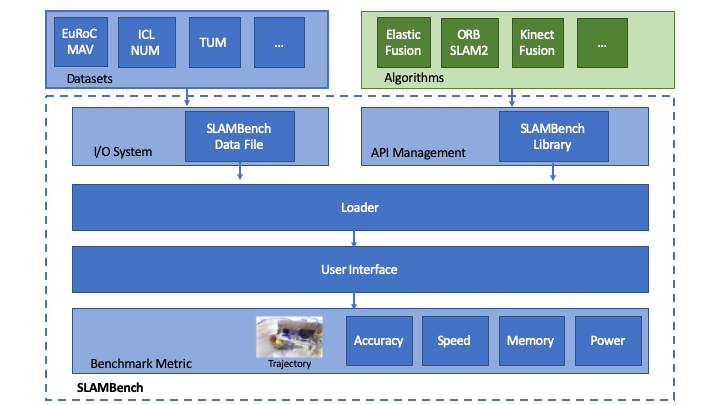
\includegraphics[width=14cm]{figures/slambench-architecture.png}
	\centering
\end{figure}

\subsubsection*{I/O – Data Ingestion System}

If the SLAMBench directly ingest datasets from various sources that may have different data formats and file types, it would be hard to allow different algorithms to perform benchmarking on the same dataset. Without multiple data formats available for the dataset, comparison between different algorithms would not be possible. Hence, I/O System translates different datasets into uniformly formatted SLAMBench datafiles. 
\begin{lstlisting}
DATAFILE = <HEADER><SENSORS><GT_FRAMES><IN_FRAMES>
HEADER   = <VERSION:4B><SENSOR_COUNT:4B>
SENSORS  = <SENSOR 1>...<SENSOR N>
SENSOR   = <TYPE:4B><PARAMETERS>
GT_FRAMES= <EMPTY>|<GT_FRAME 1>...<GT_FRAME N>
IN_FRAMES= <IN_FRAME 1>...<IN_FRAME N>
GT_FRAME = <TIMESTAMP:8B><GT_TYPE:4B><DATA>
IN_FRAME = <TIMESTAMP:8B><IN_TYPE:4B><DATA>
GT_TYPE  = POSE|POINT_CLOUD
IN_TYPE  = RGB_FRAME|DEPTH_FRAME|IMU_FRAME|...
\end{lstlisting}

By doing so, integrating new dataset will be seamless as long as the input frame types (\code{IN\_FRAMES}) are supported by the collection of helper functions for various sensor types (indicated in the \code{SENSOR} object), including RGB, greyscale, depth images, IMU data and pixel events. 
SLAMBench data file also allows users to input ground truth (\code{GT\_FRAME} and \code{GT\_TYPE} as pose or point cloud) for each frame, so that these parameters can later be utilized for the accuracy evaluation. 

\subsubsection*{API – Library Integration }
The main challenge for SLAMBench is to integrate different SLAM algorithms that exist in various libraries. 
Most libraries do not conform to the same API format, preventing SLAMBench from directing interfacing with all of them. 
Therefore, in SLAMBench, a standalone API, along with a collection of helper objects, is created to interface with SLAM algorithms in different libraries. 
This API functionally abstract the general process of a SLAM algorithm into three phases: initializing, processing, and finalizing phases. 

\begin{figure}[h]
	\caption{API Workflow \cite{bodin2018slambench2}}
	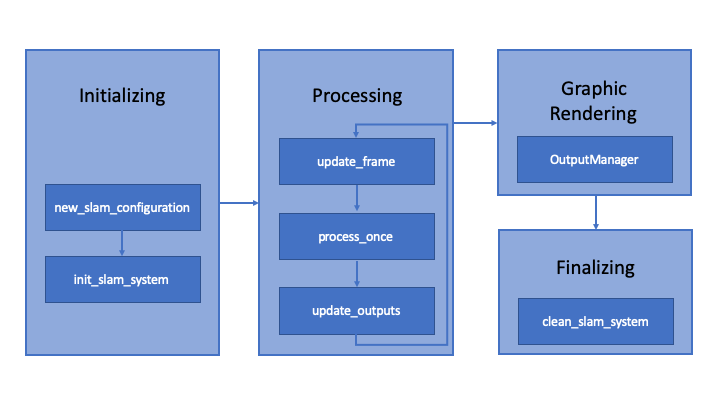
\includegraphics[width=14cm]{figures/api-workflow.png}
	\centering
\end{figure}

In the initializing phase, \code{sb\_new\_slam\_configuration} sets the user configuration for the SLAM algorithm. 
Then \code{sb\_init\_slam\_system} initializes the SLAM system with certain memory allocation. 
In the processing phase, \code{sb\_update\_frame} will deliver the frame to SLAM algorithm and let the algorithm to compute the framework with \code{sb\_process\_once} function. 
Afterwards, estimation of pose and mapping is obtained through \code{sb\_update\_outputs}. 
Finally, in the finalizing phase, after all frames have been processed, \code{sb\_clean\_slam\_system} release the previously allocated memory. 
Mapping rendering and extraction are complex, as the method is required to deal with a large number of different data structures. 
Since this part is not directly related to the filtering system, I will not discuss this part in detail.

\subsubsection*{Loader}
Loader is a crucial middleware that connect everything together and execute the experiment. 
It is the main program that ingests the SLAMBench data files translated by the I/O System, triggers the loop which sends each frame to the SLAM algorithms, and outputs the trajectory map. 

\subsubsection*{User Interface}
The user interface produces the mapping result and benchmark metrics, including trajectory, accuracy, reconstruction, power consumption, memory usage etc. 
The GUI uses Pangolin library to provide a visualization of trajectory, point cloud and ground truth. The text interface produces other non-visual metrics.

\subsection{Strengths of SLAMBench Architecture}
There are a few strengths that make SLAMBench stand out from other benchmarking tools for SLAM systems: extensibility, centralized configuration, and modularity. 

\subsubsection*{Extensibility with Multiple Datasets}
By having a I/O system that can convert different data frames into a unified SLAMBench data files, SLAMBench is able to ingest any type of datasets that are in different formats, including ICL-NUIM, TUM RGB-D, and EuRoC MAV. 
Even the new dataset may contain frames that are not able to be ingested by current sensor types in SLAMBench, SLAMBench allows the user to extend the library to accommodate any kind of sensor format. 

\subsubsection*{Centralized Configuration for Various Algorithms}
Since the API management system of SLAMBench extrapolates the generic process of SLAM systems, SLAMBench, together with the collection of helper objects specific to each SLAM system, is able to interface with multiple types of algorithms, resulting in centralized configuration for the user in a single general API. 
New SLAM system can also be integrated through connecting its specific API with the API of SLAMBench. 

\subsubsection*{Modularity of the Framework}
The framework of SLAMBench is highly modular, as each part of system performs dedicated functions. 
I/O system for dataset ingestion, API management for SLAM system integration, Loader, and User Interface are all separated functions that allow researchers to modified one part of the system without changing the whole structure. 
In addition, modularity is also exhibited in each part of the system itself: I/O system is able to call different sensor types for different data frames; API management allows changes for one SLAM system without impacting others; User interface enables the user to change the default Pangolin library \cite{Pangolin} to other visualization tool such as ROS visualizer \cite{ROS}.  

\subsection{Weaknesses and Obstacles}
However, there are also some weaknesses of the framework that brings us obstacles to integrate the new filtering system to SLAMBench.

\subsubsection*{Singular \& Nonconcurrent Data Pipeline}
Currently, the data ingestion process is a for-loop that iteratively ingest frame (SLAM data file) one by one. 
Specific sensor type will then be trigged to process the frame and send the data to SLAM algorithm for further processing and estimation. 
However, such singular, nonconcurrent data pipelining is different from how actually multiple sensors ingest data during mapping and localization. 
In reality, the processing of frames is asynchronous, as each sensor performs independently to ingest, process and deliver data to the SLAM system. 

\begin{figure}[h]
	\caption{Example of Singular and Concurrent Input Stream}
	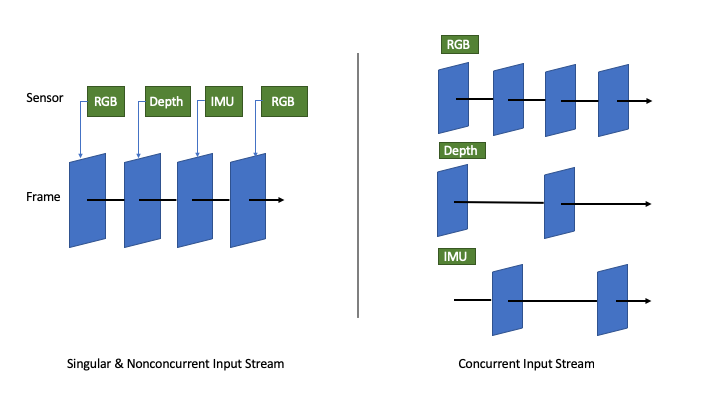
\includegraphics[width=14cm]{figures/concurrency.png}
	\centering
\end{figure}

The simple, singular frame input stream may perform properly without any problem if a combined computational task of frames from multiple various sensors is not required.  
However, some scenarios, such as the filtering system I intend to construct, require frames from multiple sensors at the same time to perform statistical analysis. 
For example, for the filtering system to drop frames from both the RGB sensor and depth sensor, a combined analysis of previous and current frames from both RGB and depth sensors is required to make a drop decision. 
A singular input stream of frames would not enable such analysis unless some data buffering mechanism is built.

\subsubsection*{Pre-determined Sensor Setting}

Until now the sensor configuration has been predetermined by the initial input frame. 
For example, if the input RGB frame is $250 \times 250$, then the RGB sensor object will exclusively process the frame at $250 \times 250$. 
This static configuration is not a problem if the specification of the input frame does not change in the run time. 
However, if a filtering system is put in place to change the size of each frame at the run time, then statically configured sensor object would not be able to properly ingest the resized frame.

\subsubsection*{Difficult Installation and Interaction}
Installation of SLAMBench is not a smooth process because the framework relies on specific and multiple dependencies. 
There is no integrated installer for SLAMBench framework, which would allow the user to perform one-click installation. 
There is an attempt to allow users to download all dependencies through \code{make dep}, but unfortunately, \code{make dep} does not perform properly until the time of writing this paper. 
In addition, although the configuration of all SLAM system is done through centralized API, for someone who is not familiar with SLAMBench, it is still troublesome to navigate and set specific configurations through terminal.
